%HW08.tex
%
% Eighth Homework for Graduate Algebra
% Frank Sottile
%%%%%%%%%%%%%%%%%%%%%%%%%%%%%%%%%%%%%%%%%%%%%%%%%%%%%%%%%%%%%%%%%%%%%%%
\documentclass[12pt]{article}
\usepackage{multicol,amssymb,amsmath}
\usepackage{colordvi,graphicx}

%%%%%%%%%%%%%%%%%%%%%%%%%%%%%%%%  Layout     %%%%%%%%%%%%%%%%%%%%%%%%%%%%%%%%%%%%%%
\usepackage{vmargin}
\setpapersize{USletter}
\setmargrb{0.5cm}{0.05cm}{0.5cm}{0.05cm} % --- sets all four margins LTRB

\pagestyle{empty}

%%%%%%%%%%%%%%%%%%%%%%%%%%%%%%%%%%%%%%%%%%%%
\newcommand{\CC}{{\mathbb C}}
\newcommand{\KK}{{\mathbb K}}
\newcommand{\NN}{{\mathbb N}}
\newcommand{\QQ}{{\mathbb Q}}
\newcommand{\RR}{{\mathbb R}}
\newcommand{\TT}{{\mathbb T}}
\newcommand{\ZZ}{{\mathbb Z}}

\newcommand{\calA}{{\mathcal A}}
\newcommand{\bfe}{{\bf e}}
\newcommand{\bfi}{{\bf i}}
\newcommand{\bfj}{{\bf j}}

\newcommand{\Hom}{\mbox{Hom}}
\newcommand{\spec}{\mbox{spec}}
\newcommand{\cone}{\mbox{cone}}

\newcommand{\vect}[2]{(\begin{smallmatrix}#1\\#2\end{smallmatrix})}
\newcommand{\msp}{\hspace{8pt}}

\newcommand{\Square}{\raisebox{-2pt}{\includegraphics{images/Square.eps}}}


\def\Color#1#2{\special{color push cmyk #1}#2\special{color pop}}
%\def\Indigo#1{\Color{.42 1. 0. .49}{#1}}
\def\Indigo#1{\Color{1. .95 .05 .4}{#1}}
\def\MyViolet#1{\Color{.6 1. 0. .15}{#1}}


\newcommand{\barsl}{\noindent\begin{minipage}[t]{590pt}
 \Indigo{\rule{590pt}{1.2pt}}\vspace{-5.7mm}\\
\MyViolet{\rule{590pt}{1.2pt}}\vspace{-5.7mm}\\
\Blue{\rule{590pt}{1.2pt}}\vspace{-5.7mm}\\
\Green{\rule{590pt}{1.2pt}}\vspace{-5.7mm}\\
\Yellow{\rule{590pt}{1.2pt}}\vspace{-5.7mm}\\
\Orange{\rule{590pt}{1.2pt}}\vspace{-5.7mm}\\
\Red{\rule{590pt}{1.2pt}}\bigskip
\end{minipage}}


\newcommand{\barsn}{\noindent\begin{minipage}[t]{590pt}
\Indigo{\rule{590pt}{1.1pt}}\vspace{-4.5mm}\\
\MyViolet{\rule{590pt}{1.1pt}}\vspace{-4.5mm}\\
\Blue{\rule{590pt}{1.1pt}}\vspace{-4.5mm}\\
\Green{\rule{590pt}{1.1pt}}\vspace{-4.5mm}\\
\Yellow{\rule{590pt}{1.1pt}}\vspace{-4.5mm}\\
\Orange{\rule{590pt}{1.1pt}}\vspace{-4.5mm}\\
\Red{\rule{590pt}{1.1pt}}\bigskip
\end{minipage}}

\def\demph#1{\Maroon{{\sl #1}}}
\def\defcolor#1{\Maroon{#1}}

\begin{document}
\LARGE \noindent
Algebra \ \ Autumn 2023\vspace{1pt}\\
Frank Sottile\vspace{1pt}\\
\Large 16 October 2023 \hfill
\sf
 Eighth Homework\makebox[40pt][l]{\ }
\large\vspace{10pt}

\noindent
Write your answers neatly, in complete sentences.  
I highly recommend recopying your work before handing it in.
Correct and crisp proofs are greatly appreciated; oftentimes your work can be shortened and made clearer.

\barsl

\noindent\Maroon{{\large\sf Hand in for the grader Monday 23 October:}}
%\Blue{(Have this separate from \#?.)}\bigskip


\begin{enumerate}
\setcounter{enumi}{31}


%%%%%%%%%%%%%%%%%%%%%%%%%%%%%%%%%%%%%%%%%%%%%%%%%%%%%%%%%%%%%%%%%%%%%%%%%%%%%%%%%%%%%%%%%%%%%%%%%%%%
%2013, 2023
\item  
    How many elements of order seven are there in a simple group of order 168?\vspace{-2pt}
%%%%%%%%%%%%%%%%%%%%%%%%%%%%%%%%%%%%%%%%%%%%%%%%%%%%%%%%%%%%%%%%%%%%%%%%%%%%%%%%%%%%%%%%%%%%%%%%%%%%  



%%%%%%%%%%%%%%%%%%%%%%%%%%%%%%%%%%%%%%%%%%%%%%%%%%%%%%%%%%%%%%%%%%%%%%%%%%%%%%%%%%%%%%%%%%%%%%%%%%%%
% 2017 
\item   Show that any group of order 200 must contain a normal Sylow $p$-subgroup, and hence is not simple.
%%%%%%%%%%%%%%%%%%%%%%%%%%%%%%%%%%%%%%%%%%%%%%%%%%%%%%%%%%%%%%%%%%%%%%%%%%%%%%%%%%%%%%%%%%%%%%%%%%%%  


%%%%%%%%%%%%%%%%%%%%%%%%%%%%%%%%%%%%%%%%%%%%%%%%%%%%%%%%%%%%%%%%%%%%%%%%%%%%%%%%%%%%%%%%%%%%%%%%%%%%  
\item
    Recall that the quaternion group is $Q=\{\pm1,\pm i, \pm j, \pm k\}$ with $i^2=j^2=k^2=ijk=-1$ and $ij=-ji$, and etc.
    What is the center $C(Q)$ of $Q$?
    Show that $Q/C(Q)$ is abelian.
%%%%%%%%%%%%%%%%%%%%%%%%%%%%%%%%%%%%%%%%%%%%%%%%%%%%%%%%%%%%%%%%%%%%%%%%%%%%%%%%%%%%%%%%%%%%%%%%%%%%  


%%%%%%%%%%%%%%%%%%%%%%%%%%%%%%%%%%%%%%%%%%%%%%%%%%%%%%%%%%%%%%%%%%%%%%%%%%%%%%%%%%%%%%%%%%%%%%%%%%%%  
\item   Show that there is a nonabelian subgroup \defcolor{$T$} of $S_3\times \ZZ/4\ZZ$ of order 12 with generators $a,b$ such that $|a|=6$,
  $a^3=b^2$, and $ba=a^{-1}b$.

  Show that any group of order 12 with two generators satisfying these relations  is isomorphic to $T$.
%%%%%%%%%%%%%%%%%%%%%%%%%%%%%%%%%%%%%%%%%%%%%%%%%%%%%%%%%%%%%%%%%%%%%%%%%%%%%%%%%%%%%%%%%%%%%%%%%%%%  
 

%%%%%%%%%%%%%%%%%%%%%%%%%%%%%%%%%%%%%%%%%%%%%%%%%%%%%%%%%%%%%%%%%%%%%%%%%%%%%%%%%%%%%%%%%%%%%%%%%%%%  
\item   Show that the group $T$ of the previous question, $A_4$, and the dihedral group of symmetries of the regular hexagon are pairwise
  nonisomorphic. 
%%%%%%%%%%%%%%%%%%%%%%%%%%%%%%%%%%%%%%%%%%%%%%%%%%%%%%%%%%%%%%%%%%%%%%%%%%%%%%%%%%%%%%%%%%%%%%%%%%%%  
  
%%%%%%%%%%%%%%%%%%%%%%%%%%%%%%%%%%%%%%%%%%%%%%%%%%%%%%%%%%%%%%%%%%%%%%%%%%%%%%%%%%%%%%%%%%%%%%%%%%%%
\item Give a composition series for $S_4$.\vspace{-2pt}
%%%%%%%%%%%%%%%%%%%%%%%%%%%%%%%%%%%%%%%%%%%%%%%%%%%%%%%%%%%%%%%%%%%%%%%%%%%%%%%%%%%%%%%%%%%%%%%%%%%%  
  

%%%%%%%%%%%%%%%%%%%%%%%%%%%%%%%%%%%%%%%%%%%%%%%%%%%%%%%%%%%%%%%%%%%%%%%%%%%%%%%%%%%%%%%%%%%%%%%%%%%%
\item Let $p$ be a prime number.
  How many simple subgroups does $\ZZ/p\ZZ\times\ZZ/p\ZZ\times \ZZ/p\ZZ$ have?\vspace{-2pt}
%%%%%%%%%%%%%%%%%%%%%%%%%%%%%%%%%%%%%%%%%%%%%%%%%%%%%%%%%%%%%%%%%%%%%%%%%%%%%%%%%%%%%%%%%%%%%%%%%%%%  
  

\end{enumerate}
%%%%%%%%%%%%%%%%%%%%%%%%%%%%%%%%%%%%%%%%%%%%%%%%%%%%%%%%%%%%%%%%%%%%%%%%%%%%%%%%%%%%%%%%%%%%%%%%%%%%

\end{document}

\noindent\Maroon{{\large\sf Hand in to Frank Monday 2 October:}}  \Blue{(Have this on a separate sheet of paper.)}
\setcounter{enumi}{15}
\begin{enumerate}
      
%%%%%%%%%%%%%%%%%%%%%%%%%%%%%%%%%%%%%%%%%%%%%%%%%%%%%%%%%%%%%%%%%%%%%%%%%%%%%%%%%%%%%%%%%%%%%%%%%%%%  
\item     
%%%%%%%%%%%%%%%%%%%%%%%%%%%%%%%%%%%%%%%%%%%%%%%%%%%%%%%%%%%%%%%%%%%%%%%%%%%%%%%%%%%%%%%%%%%%%%%%%%%%
 
\end{enumerate}  
  
\barsl
